
% !TEX TS-program = xelatex
\documentclass[12pt,a4paper]{article}
\usepackage{fontspec}
\usepackage{polyglossia}
\setmainlanguage{russian}
\setotherlanguage{english}
\setmainfont{DejaVu Serif}
\setsansfont{DejaVu Sans}
\setmonofont{DejaVu Sans Mono}
\usepackage[a4paper,margin=2.05cm]{geometry}
\usepackage{amsmath,amssymb,mathtools}
\usepackage{graphicx}
\usepackage{booktabs}
\usepackage{longtable}
\usepackage{array}
\usepackage{hyperref}
\usepackage{caption}
\usepackage{float}
\usepackage{enumitem}
\usepackage{microtype}
\hypersetup{colorlinks=true,linkcolor=blue,urlcolor=blue}
\setlength{\parskip}{0.52em}
\setlength{\parindent}{0pt}
\renewcommand{\arraystretch}{1.12}
\sloppy

\title{\textbf{Computational Validation of Adaptive Interface Control in TMI Quantum Systems}\\
\large Расширенный отчёт по вычислительным тестам 1--22}
\author{Salkutsan Aleksey}
\date{6 мая 2026}

\begin{document}
\maketitle

\begin{abstract}
Этот отчёт объединяет вычислительную линию Tests 1--22 для прикладного квантового модуля Теории многообразных интерфейсов (ТМИ). Первоначальная линия Tests 1--11 проверяла рост $T_2^{eff}$ и $P_{success}$, затем воспроизводимость и независимую реализацию были добавлены в Tests 12--13. Tests 14--19 исследуют типы шума, восстановление amplitude damping, классификацию шума, online drift, задержанную обратную связь и оптимизацию latency-aware политики. Tests 20--22 переводят управление из single-metric режима к cost boundary и multi-objective boundary manifold.

Главная проверяемая цепочка остаётся узкой:
\[
I_Q^{coh-auto}\Rightarrow T_2^{eff}\uparrow\Rightarrow P_{success}\uparrow.
\]
Новая расширенная цепочка:
\[
\text{single metric}\to\text{cost boundary}\to\text{multi-objective boundary manifold}.
\]
Это не лабораторное доказательство существования $\Xi_I^{auto}$, а воспроизводимая вычислительная линия проверки инженерного механизма автоинтерфейсного управления.
\end{abstract}

\tableofcontents
\newpage

\section{Статус отчёта}

Этот документ фиксирует модуль:
\[
\boxed{\text{TMI Quantum Computational Validation 0.2}}
\]
Он должен рассматриваться как Supplement к физическому слою TMI-Physics 2.2, а не как самостоятельное доказательство всей теории.

Главная позитивная формула:
\[
\boxed{I_Q^{coh-auto}\Rightarrow T_2^{eff}\uparrow\Rightarrow P_{success}\uparrow}
\]
Главная отрицательная формула:
\[
\boxed{\operatorname{AutoInterface}\not\Rightarrow\operatorname{SafeInterface}}
\]
Главная новая формула Tests 20--22:
\[
\boxed{\operatorname{AutoInterface}+\operatorname{BoundaryManifoldDetection}\Rightarrow\operatorname{ManifoldAdaptiveControl}}
\]

\section{Сводка Tests 1--22}

\begin{longtable}{p{1.0cm}p{4.2cm}p{5.0cm}p{5.1cm}}
\toprule
Test & Название & Критерий / смысл & Результат \\
\midrule
\endfirsthead
\toprule
Test & Название & Критерий / смысл & Результат \\
\midrule
\endhead
1 & Ramsey toy model & $T_2^{TMI}>T_2^{std}$ & $\Delta T_2=58.1\,\mu s$ \\
2 & Noisy Ramsey learning & $T_2^{TMI}>T_2^{std}$ & $\Delta T_2=39.3\,\mu s$ \\
3 & Small quantum circuit & $P_{TMI}>P_{std}$ & $\Delta P=0.115$ \\
4 & Stabilized interface & $P_{stab}>P_{std}$ & $\Delta P=0.026$ \\
5 & Surrogate Monte Carlo & $E[P_{TMI}]>E[P_{std}]$ & $\Delta=0.0510, Pr=0.864$ \\
6 & Ablation study & Structured adaptive control & full TMI $\Delta=0.0680$ \\
7 & Density-matrix MC & Full matrix validation & $\Delta=0.0930, Pr=0.933$ \\
8 & Cross-model validation & Multiple circuit families & $\Delta=0.0660, Pr=0.846$ \\
9 & Failure-boundary map & Weak/failure regions & failure=0, weak=6 \\
10 & Adversarial failure & Force real failure & failure cells=58 \\
11 & Safety recovery & Mitigation after failure & recovered=31/58 \\
12 & Reproducibility harness & One-command validation & passed=11/11 \\
13 & Independent simulator & Qiskit/Cirq-style check & $\Delta=0.1121, Pr=1.000$ \\
14 & Noise-model stress & Noise class robustness & passed=3/4, $\Delta=0.0068$ \\
15 & Amplitude damping recovery & $T_1$-aware layer & $\Delta_{relax}=0.1532$ \\
16 & Noise classifier & Classify then control & acc=0.952, $\Delta=0.0554$ \\
17 & Online noise drift & Dynamic reclassification & $\Delta=0.0255, acc=0.816$ \\
18 & Delayed feedback & Latency hurts online control & online=0.883, delayed2=0.861 \\
19 & Latency policy optimization & Predictive latency layer & opt=0.875 > d2=0.861 \\
20 & Cost-overhead tradeoff & Utility and efficiency & $U_{hp}=0.0705$ \\
21 & Cost-interface boundary & $B_{cost}$ & $\lambda^*=0.0636$ \\
22 & Multi-objective control & $\mathcal{{M}}_{boundary}$ & std=0.608, ca-low=0.373 \\
\bottomrule
\end{longtable}

\section{Tests 1--11: базовая линия, отказ и восстановление}

Tests 1--4 показывают переход от Ramsey-когерентности к вероятности успеха малой схемы:
\[
T_2^{eff}\uparrow\Rightarrow P_{success}\uparrow.
\]
Tests 5--8 показывают статистическую устойчивость: surrogate Monte Carlo, full density-matrix Monte Carlo и cross-model validation. Tests 9--11 добавляют научную честность: карта слабых зон, adversarial failure и safety-aware recovery.


% Figure omitted because source image was not present in current artifact set.



% Figure omitted because source image was not present in current artifact set.



% Figure omitted because source image was not present in current artifact set.



% Figure omitted because source image was not present in current artifact set.


\section{Tests 12--13: воспроизводимость и независимая реализация}

\subsection{Test 12: reproducibility harness}

Test 12 фиксирует репозиторный принцип:
\[
\text{one command}\Rightarrow\text{summary}\Rightarrow\text{pass/fail matrix}\Rightarrow\text{manifest}.
\]
Результат:
\[
11/11\ \text{tests passed}.
\]

\begin{figure}[H]
\centering
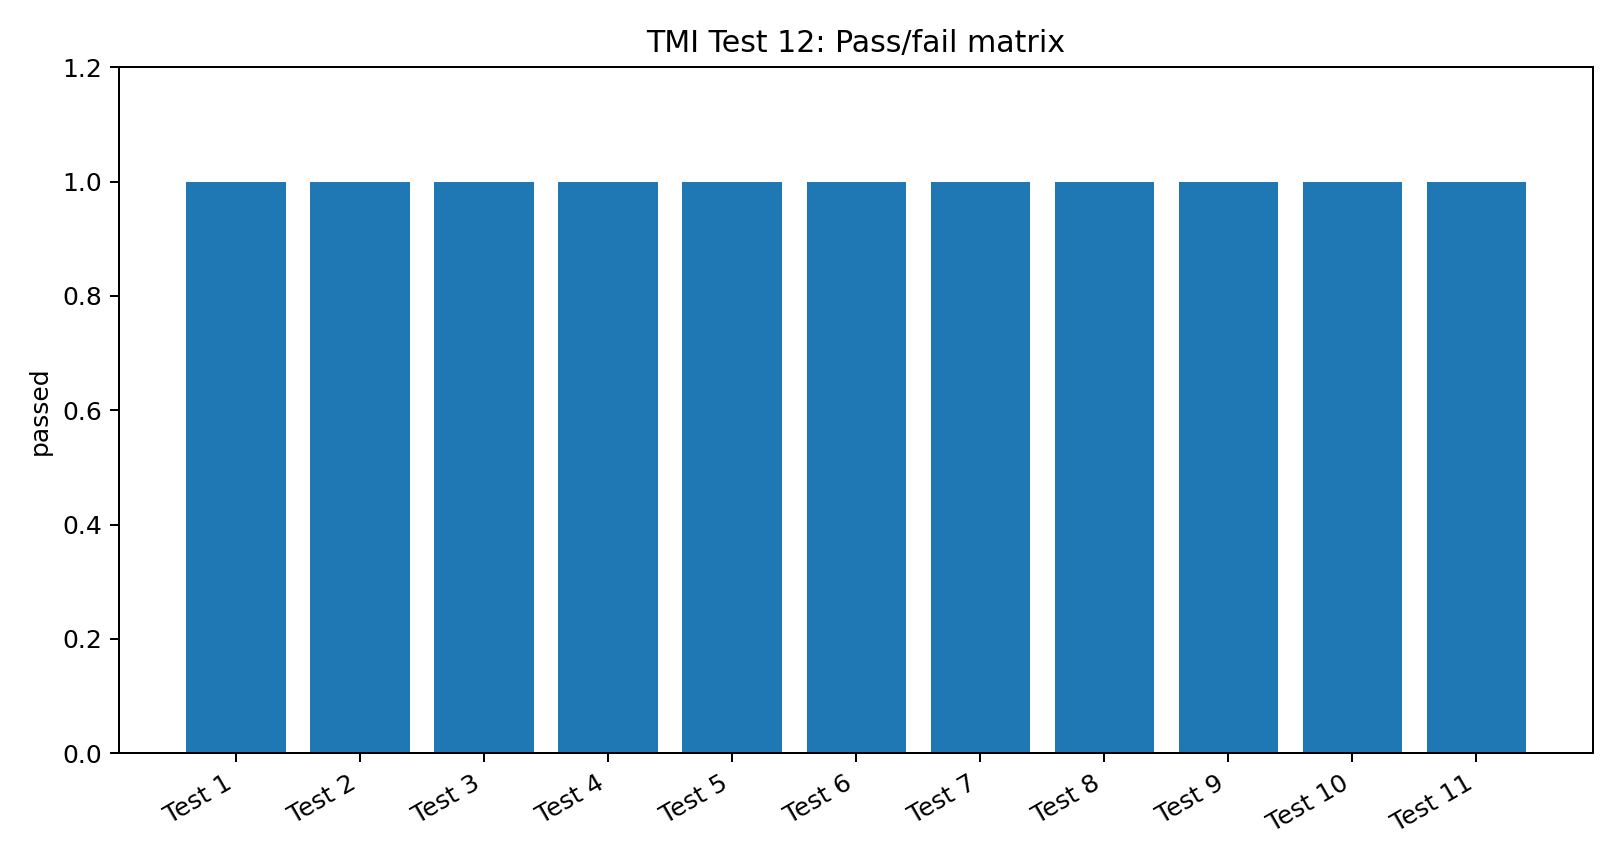
\includegraphics[width=0.82\linewidth]{figures/fig_test12_passfail.png}
\caption{Test 12: pass/fail матрица воспроизводимости.}
\end{figure}

\subsection{Test 13: independent simulator implementation}

Test 13 проверяет ключевой результат независимой Qiskit/Cirq-style реализацией. Результат:
\[
\Delta P_{TMI-std}=0.1121,\qquad Pr(P_{TMI}>P_{std})=1.000.
\]

\begin{figure}[H]
\centering
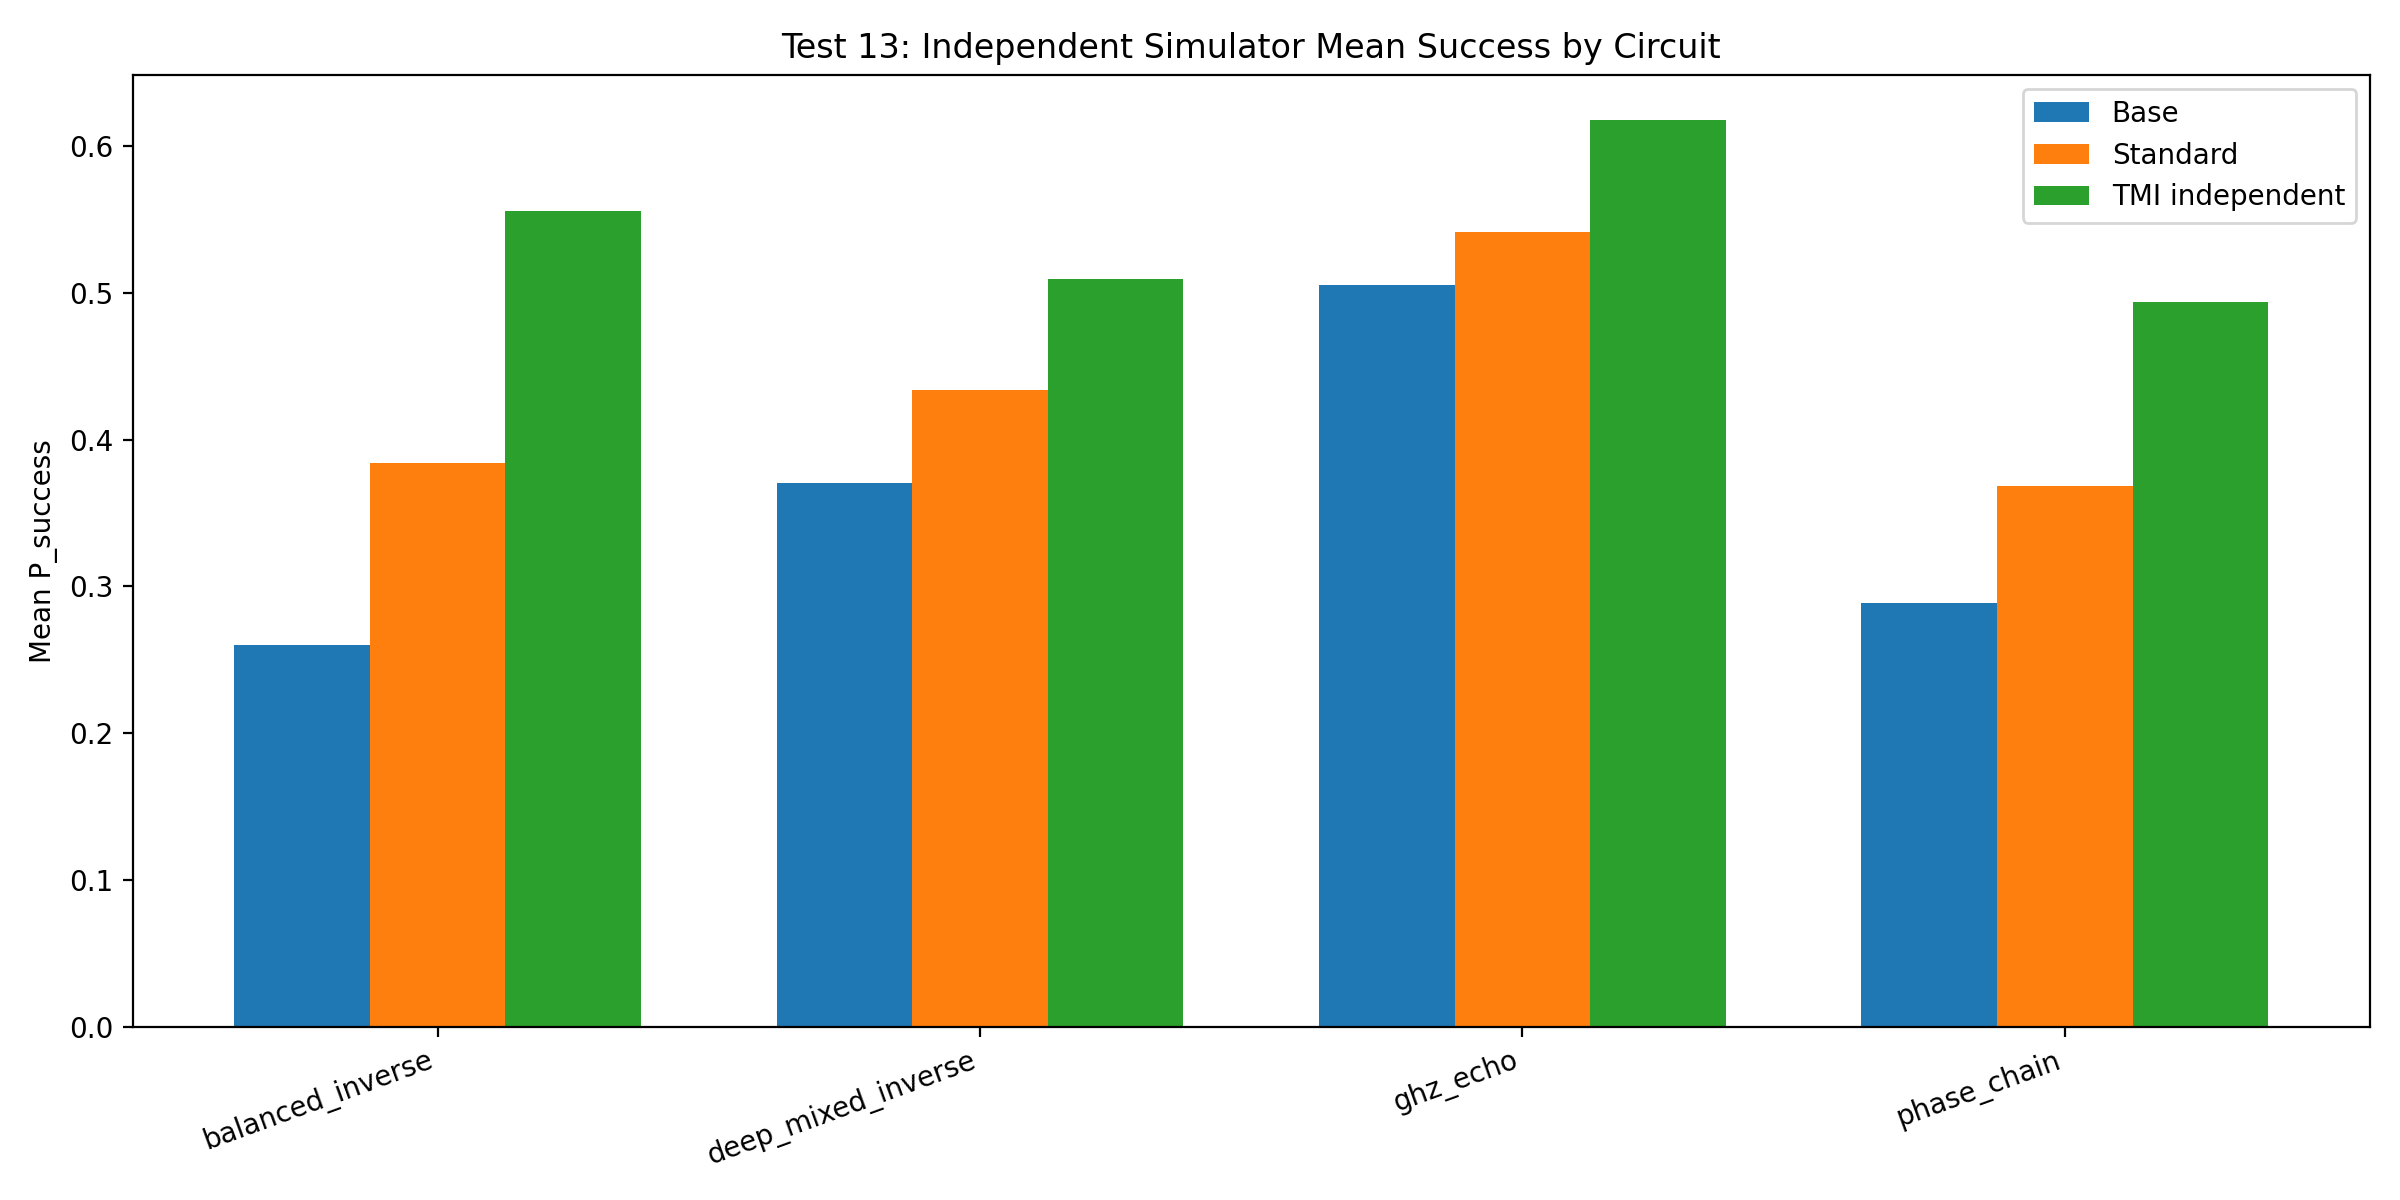
\includegraphics[width=0.88\linewidth]{figures/fig_test13_mean.png}
\caption{Test 13: независимый симулятор подтверждает выигрыш TMI.}
\end{figure}

\section{Tests 14--17: noise-specific и online adaptive interface}

Test 14 показывает, что coherence-only TMI не универсален: amplitude damping требует отдельного relaxation-aware слоя. Test 15 добавляет такой слой. Tests 16--17 развивают это в noise-classifier и online drift adaptation:
\[
NoiseFeatures\Rightarrow NoiseClass\Rightarrow ControlLayer\Rightarrow P_{success}\uparrow.
\]
Динамическая версия:
\[
NoiseClass(t)\Rightarrow ControlLayer(t)\Rightarrow OnlineAdaptiveControl.
\]

\begin{figure}[H]
\centering
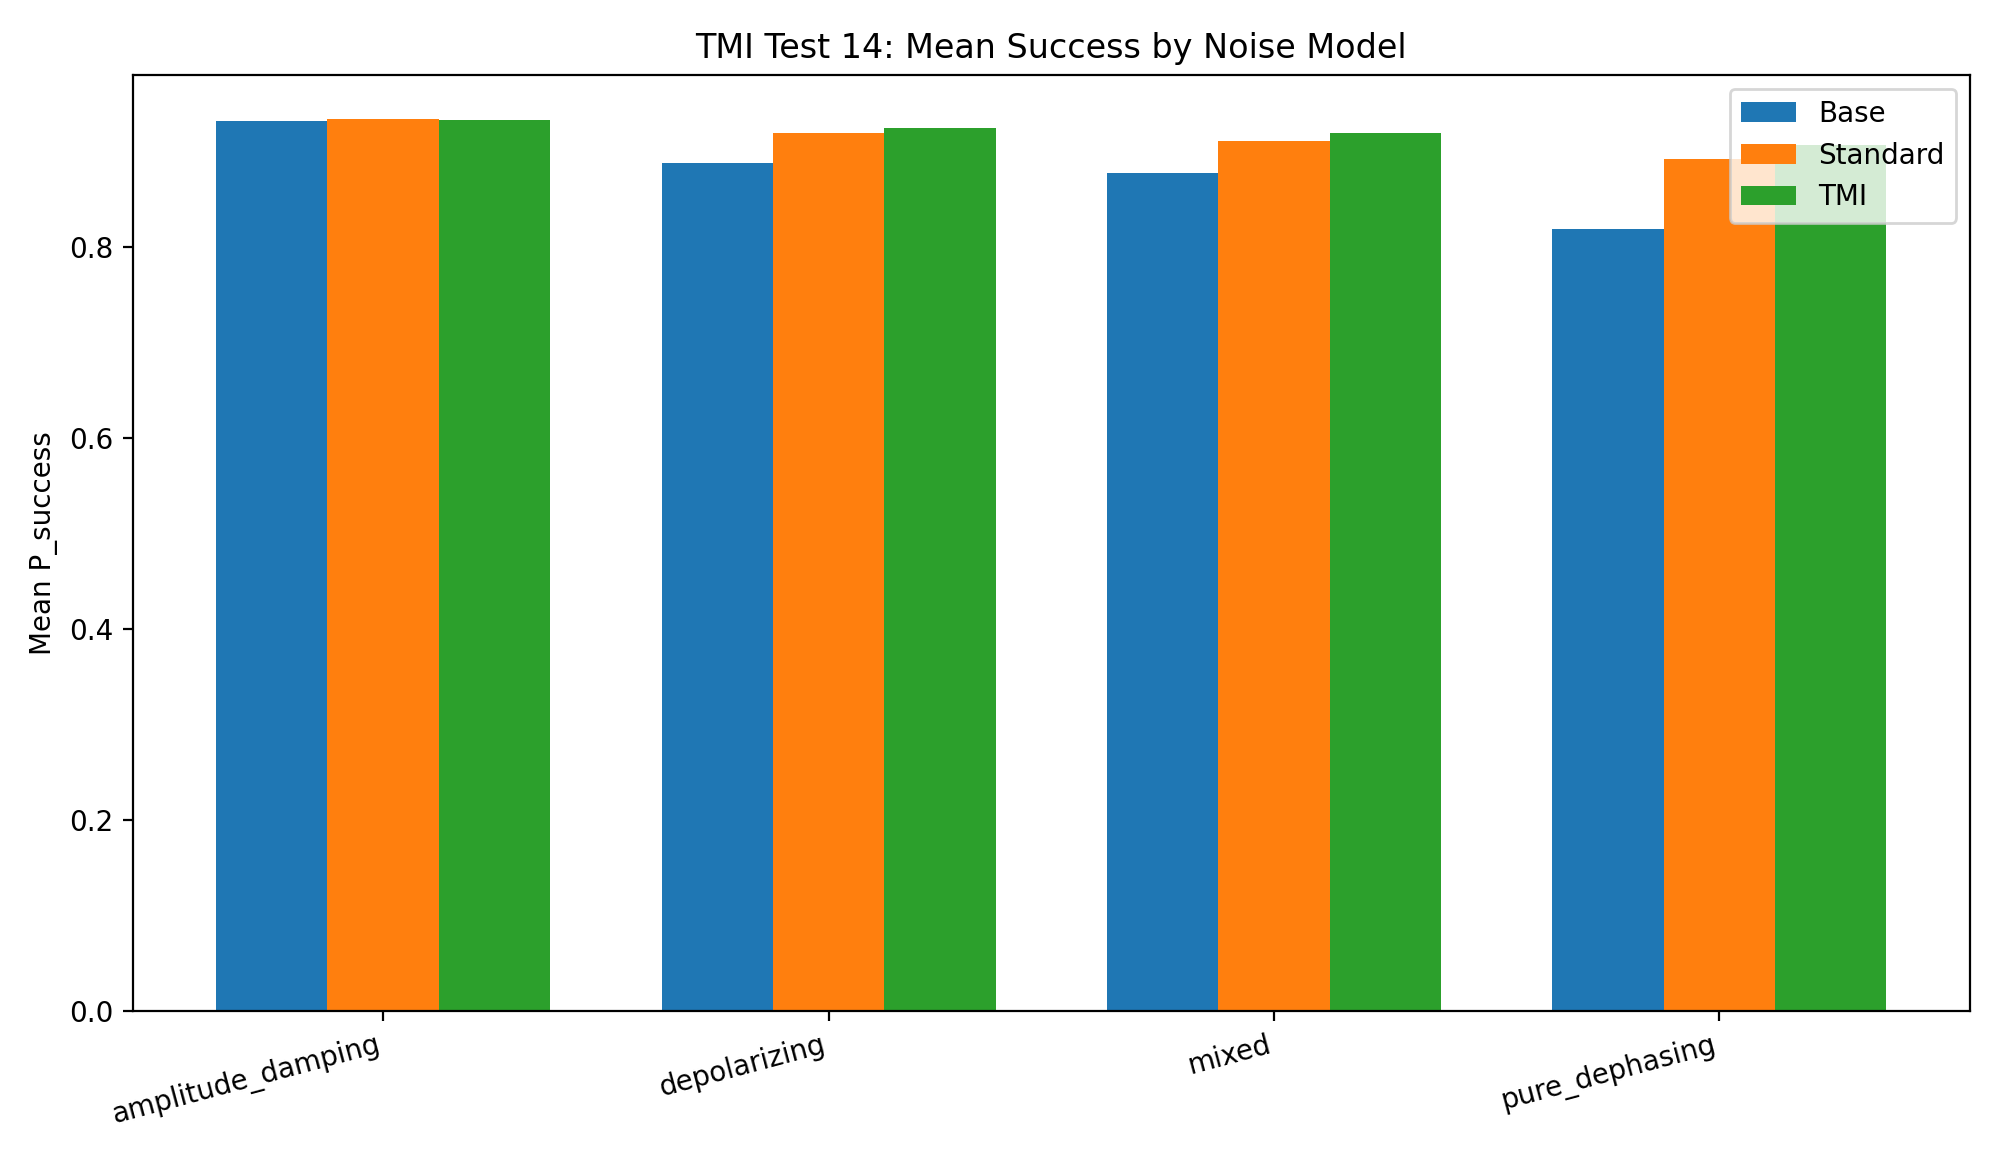
\includegraphics[width=0.86\linewidth]{figures/fig_test14_noise.png}
\caption{Test 14: stress test по типам шума. Amplitude damping выявляет ограничение coherence-only слоя.}
\end{figure}

\begin{figure}[H]
\centering
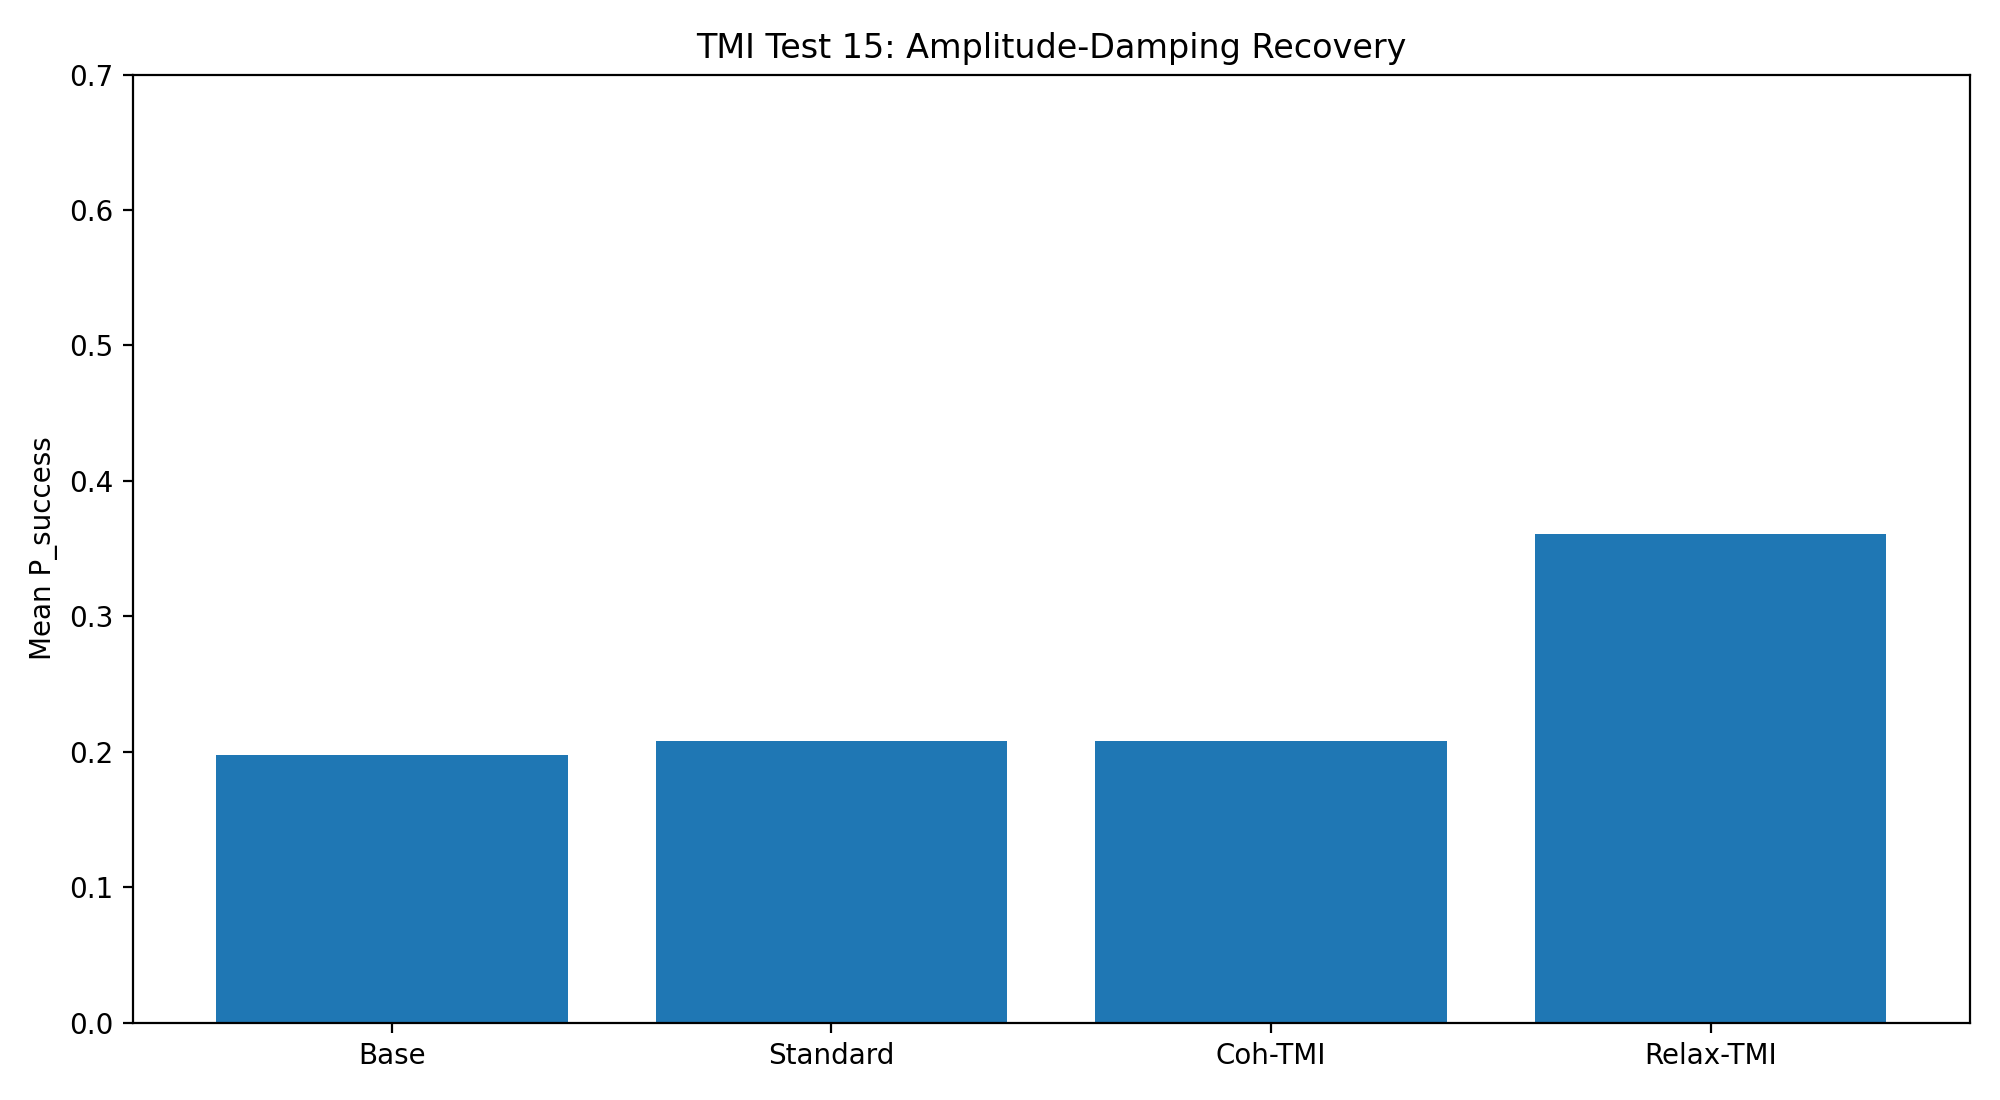
\includegraphics[width=0.78\linewidth]{figures/fig_test15_recovery.png}
\caption{Test 15: relaxation-aware слой восстанавливает выигрыш при amplitude damping.}
\end{figure}

\begin{figure}[H]
\centering
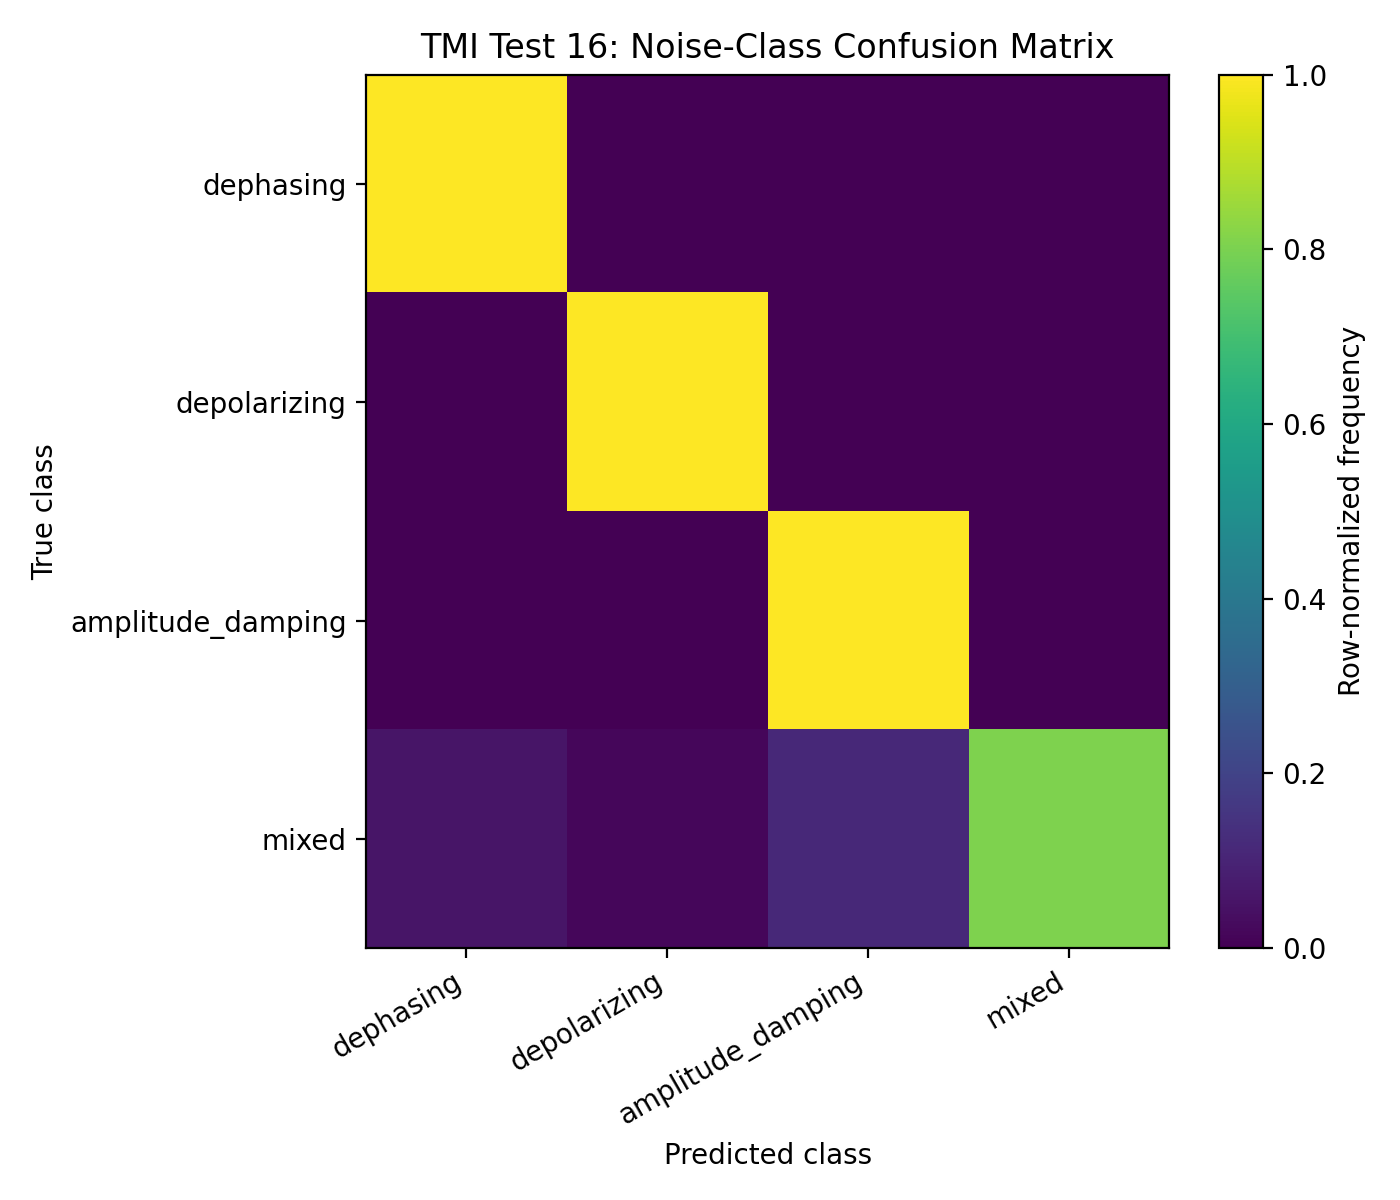
\includegraphics[width=0.72\linewidth]{figures/fig_test16_classifier.png}
\caption{Test 16: confusion matrix классификатора шума.}
\end{figure}

\begin{figure}[H]
\centering
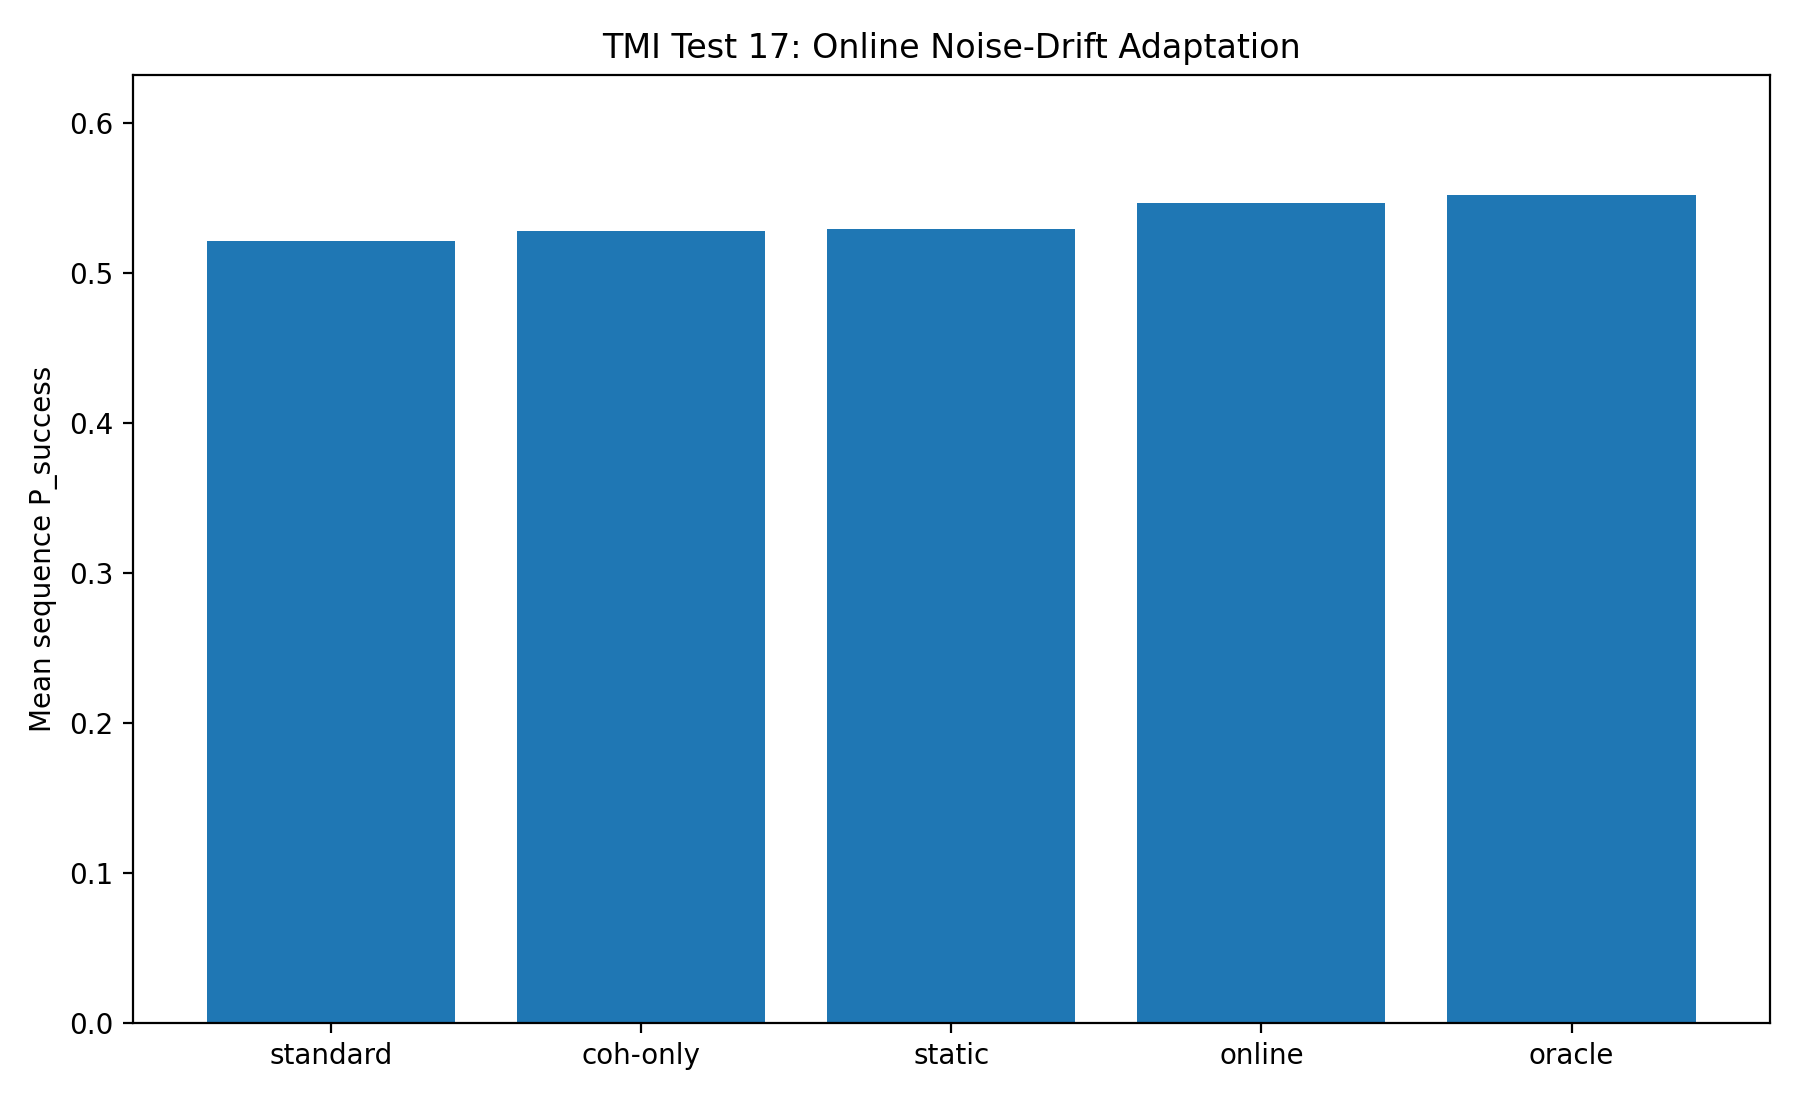
\includegraphics[width=0.82\linewidth]{figures/fig_test17_online.png}
\caption{Test 17: online classifier выигрывает у static classifier при noise drift.}
\end{figure}

\section{Tests 18--19: задержка обратной связи и latency-aware управление}

Test 18 проверяет устаревшее состояние:
\[
NoiseClass(t-\Delta t)\Rightarrow ControlLayer(t).
\]
Результат: задержка снижает качество online control:
\[
P_{online}=0.883,\qquad P_{delayed\ d2}=0.861.
\]
Test 19 улучшает latency-aware слой через predictive distribution:
\[
NoiseClass(t-\Delta t)\Rightarrow PredictiveNoiseDistribution(t)\Rightarrow ControlLayer(t).
\]
После оптимизации:
\[
P_{latency-opt}=0.875 > P_{delayed\ d2}=0.861.
\]

\begin{figure}[H]
\centering
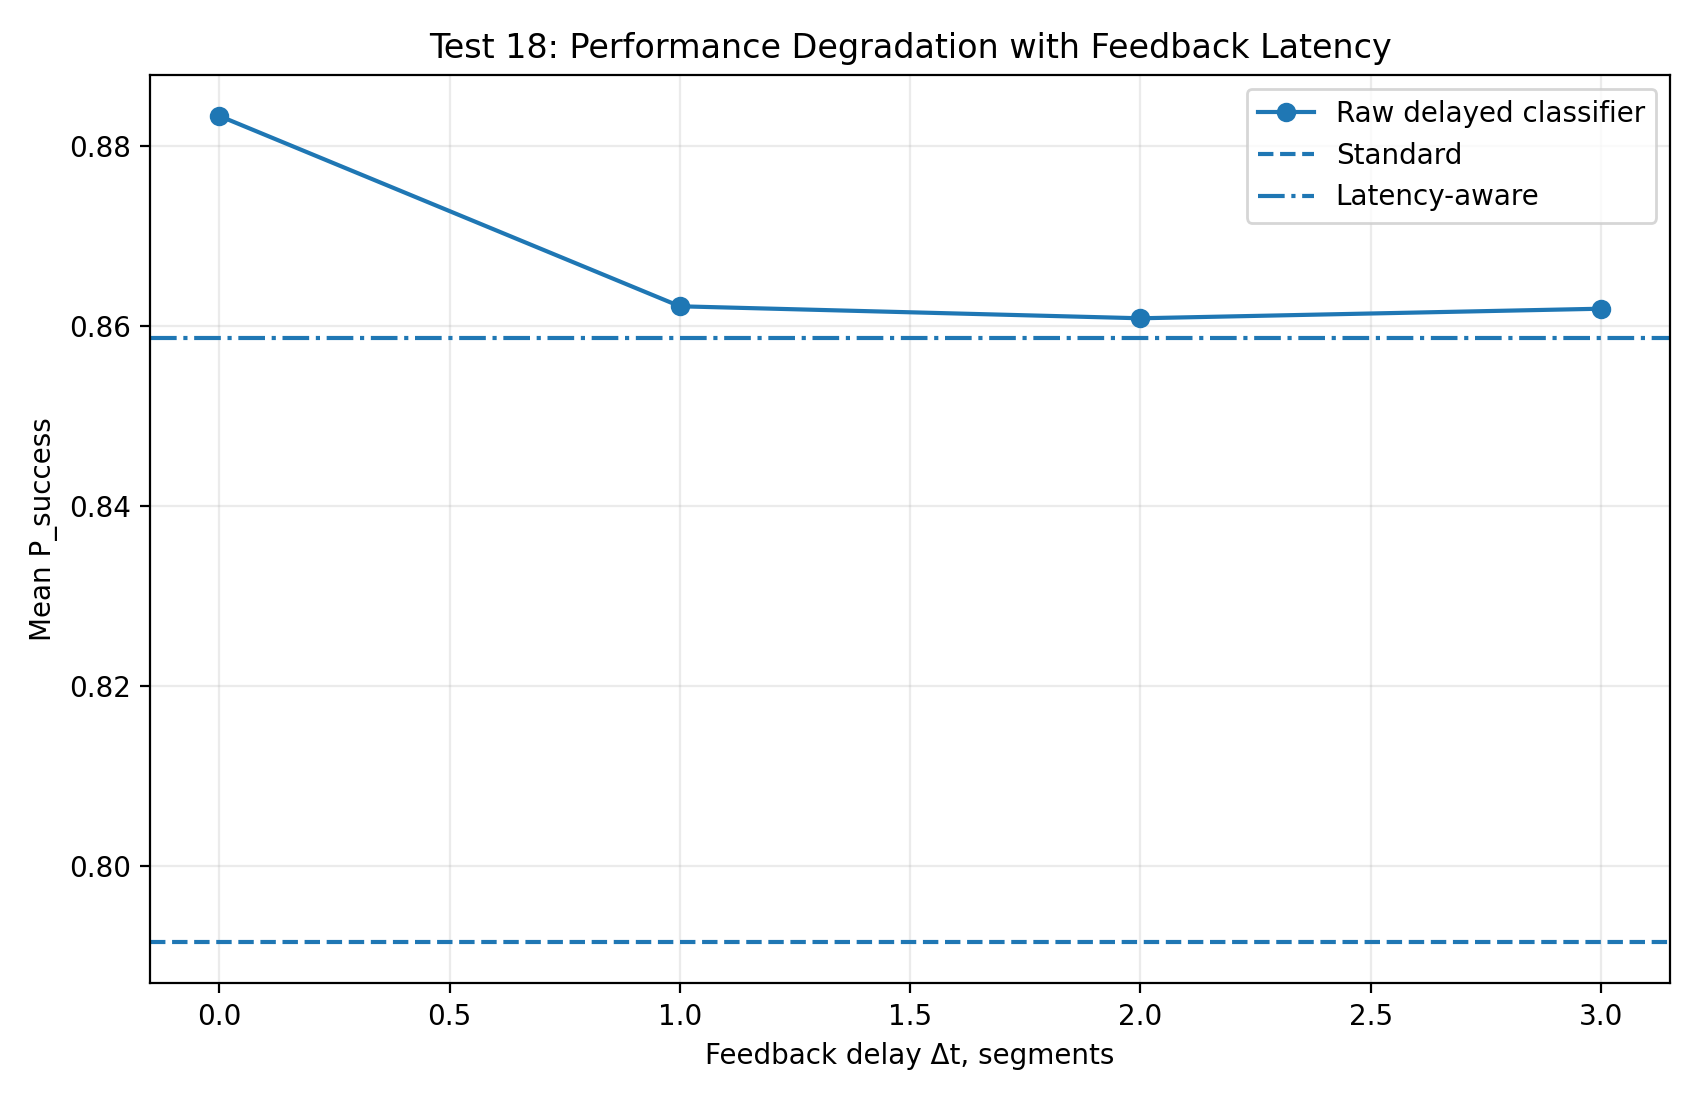
\includegraphics[width=0.82\linewidth]{figures/fig_test18_latency.png}
\caption{Test 18: деградация качества при задержке feedback.}
\end{figure}

\begin{figure}[H]
\centering
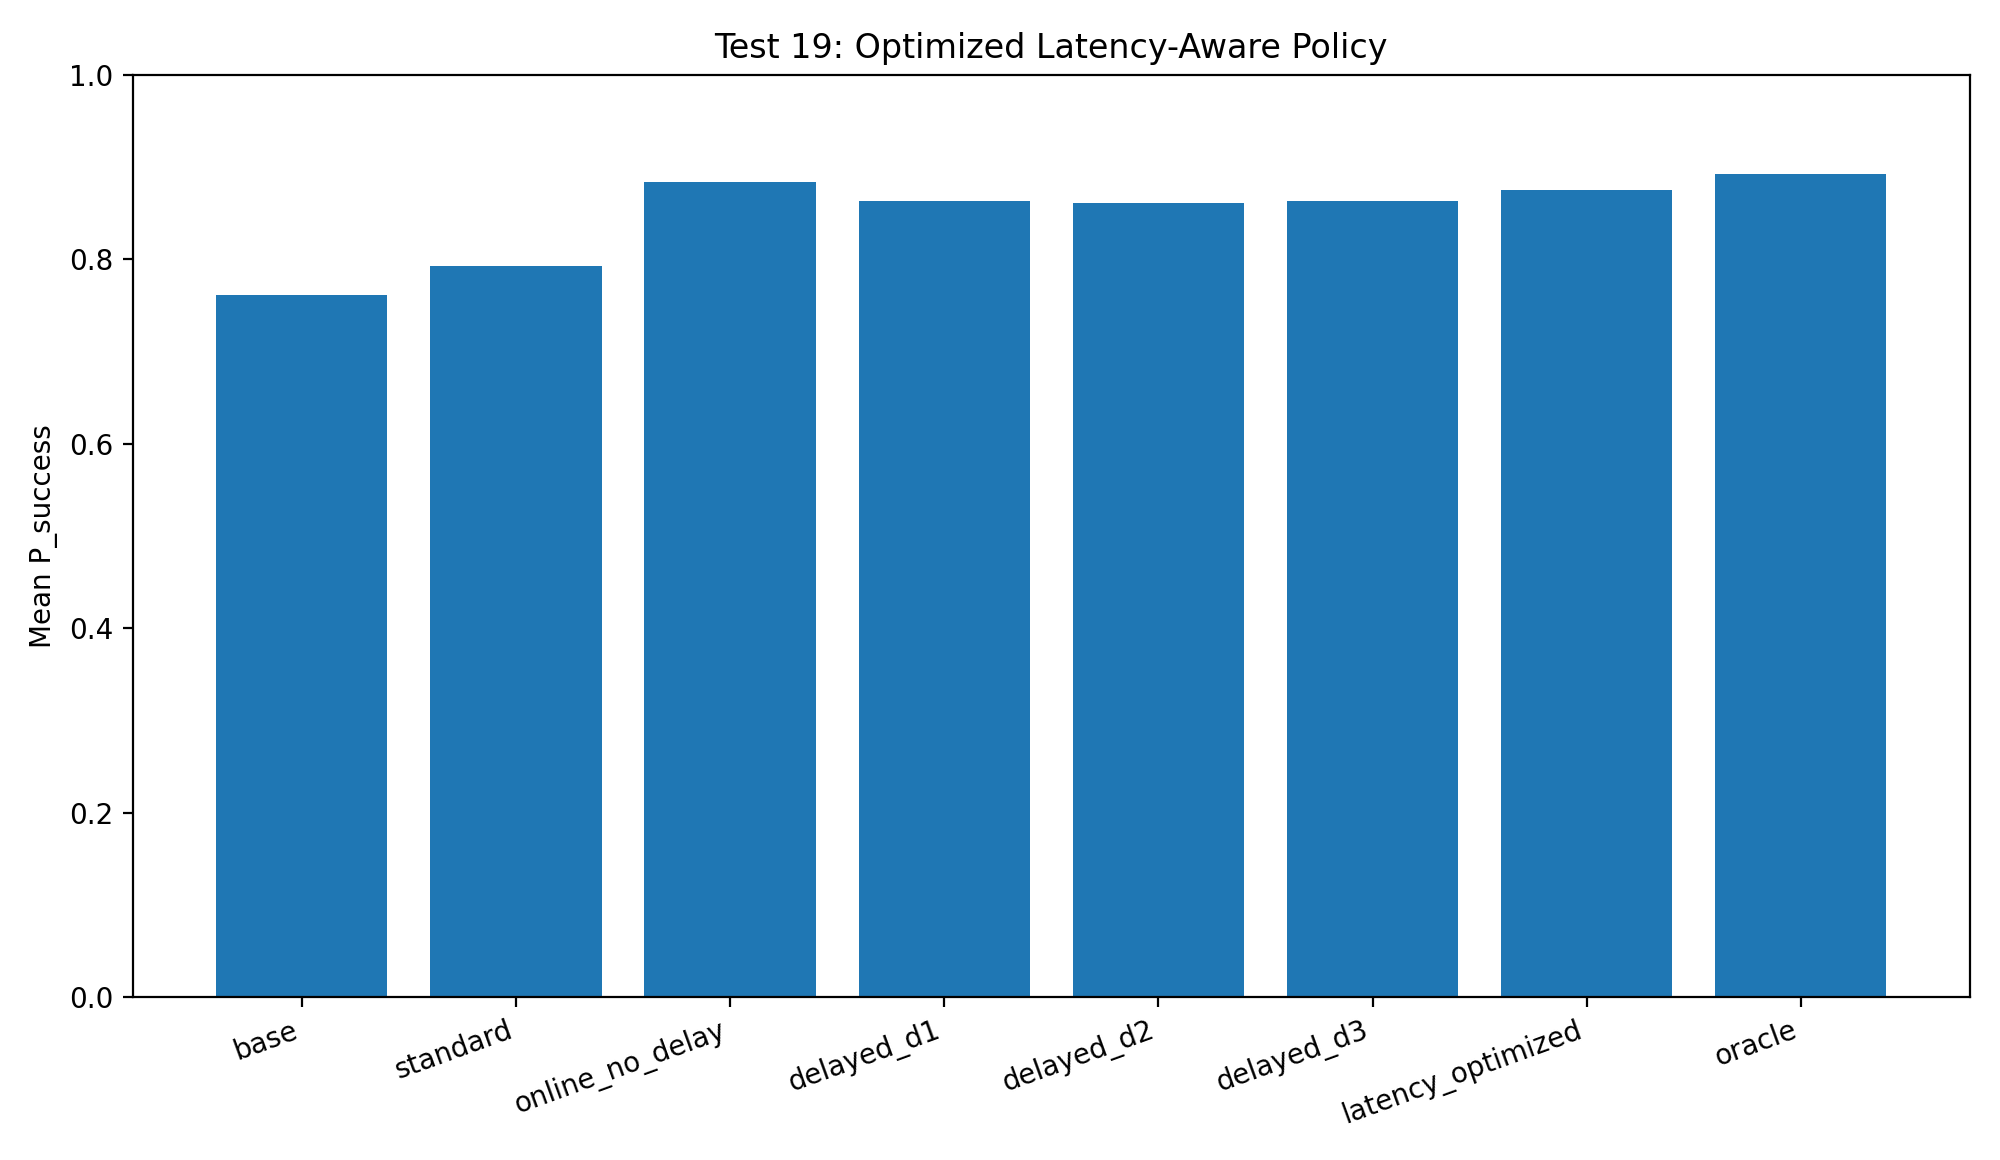
\includegraphics[width=0.82\linewidth]{figures/fig_test19_opt.png}
\caption{Test 19: оптимизированный latency-aware слой превосходит raw delayed режимы.}
\end{figure}

\section{Tests 20--22: от single metric к boundary manifold}

\subsection{Test 20: cost-overhead tradeoff}

В Test 20 вводится цена управления:
\[
Efficiency=\frac{P_{mode}-P_{standard}}{Cost_{mode}-Cost_{standard}},
\]
\[
Utility=\Delta P-0.020\cdot ExtraCost.
\]
Результат: максимальная производительность не равна максимальной эффективности.

\begin{longtable}{p{4.0cm}rrrrr}
\toprule
Policy & Mean $P$ & Cost & $\Delta P$ & Efficiency & Utility \\
\midrule
\endfirsthead
\toprule
Policy & Mean $P$ & Cost & $\Delta P$ & Efficiency & Utility \\
\midrule
\endhead
base & 0.760 & 0.100 & -0.0315 & -- & -0.0315 \\
standard & 0.791 & 0.700 & 0.0000 & -- & 0.0000 \\
cost\_aware\_low & 0.865 & 1.680 & 0.0732 & 0.0747 & 0.0536 \\
cost\_aware\_balanced & 0.872 & 2.060 & 0.0808 & 0.0594 & 0.0536 \\
latency\_optimized & 0.875 & 2.060 & 0.0833 & 0.0613 & 0.0561 \\
high\_perf\_online & 0.889 & 2.073 & 0.0979 & 0.0713 & 0.0705 \\
oracle\_high\_cost & 0.898 & 2.708 & 0.1068 & 0.0532 & 0.0666 \\
\bottomrule
\end{longtable}

\begin{figure}[H]
\centering
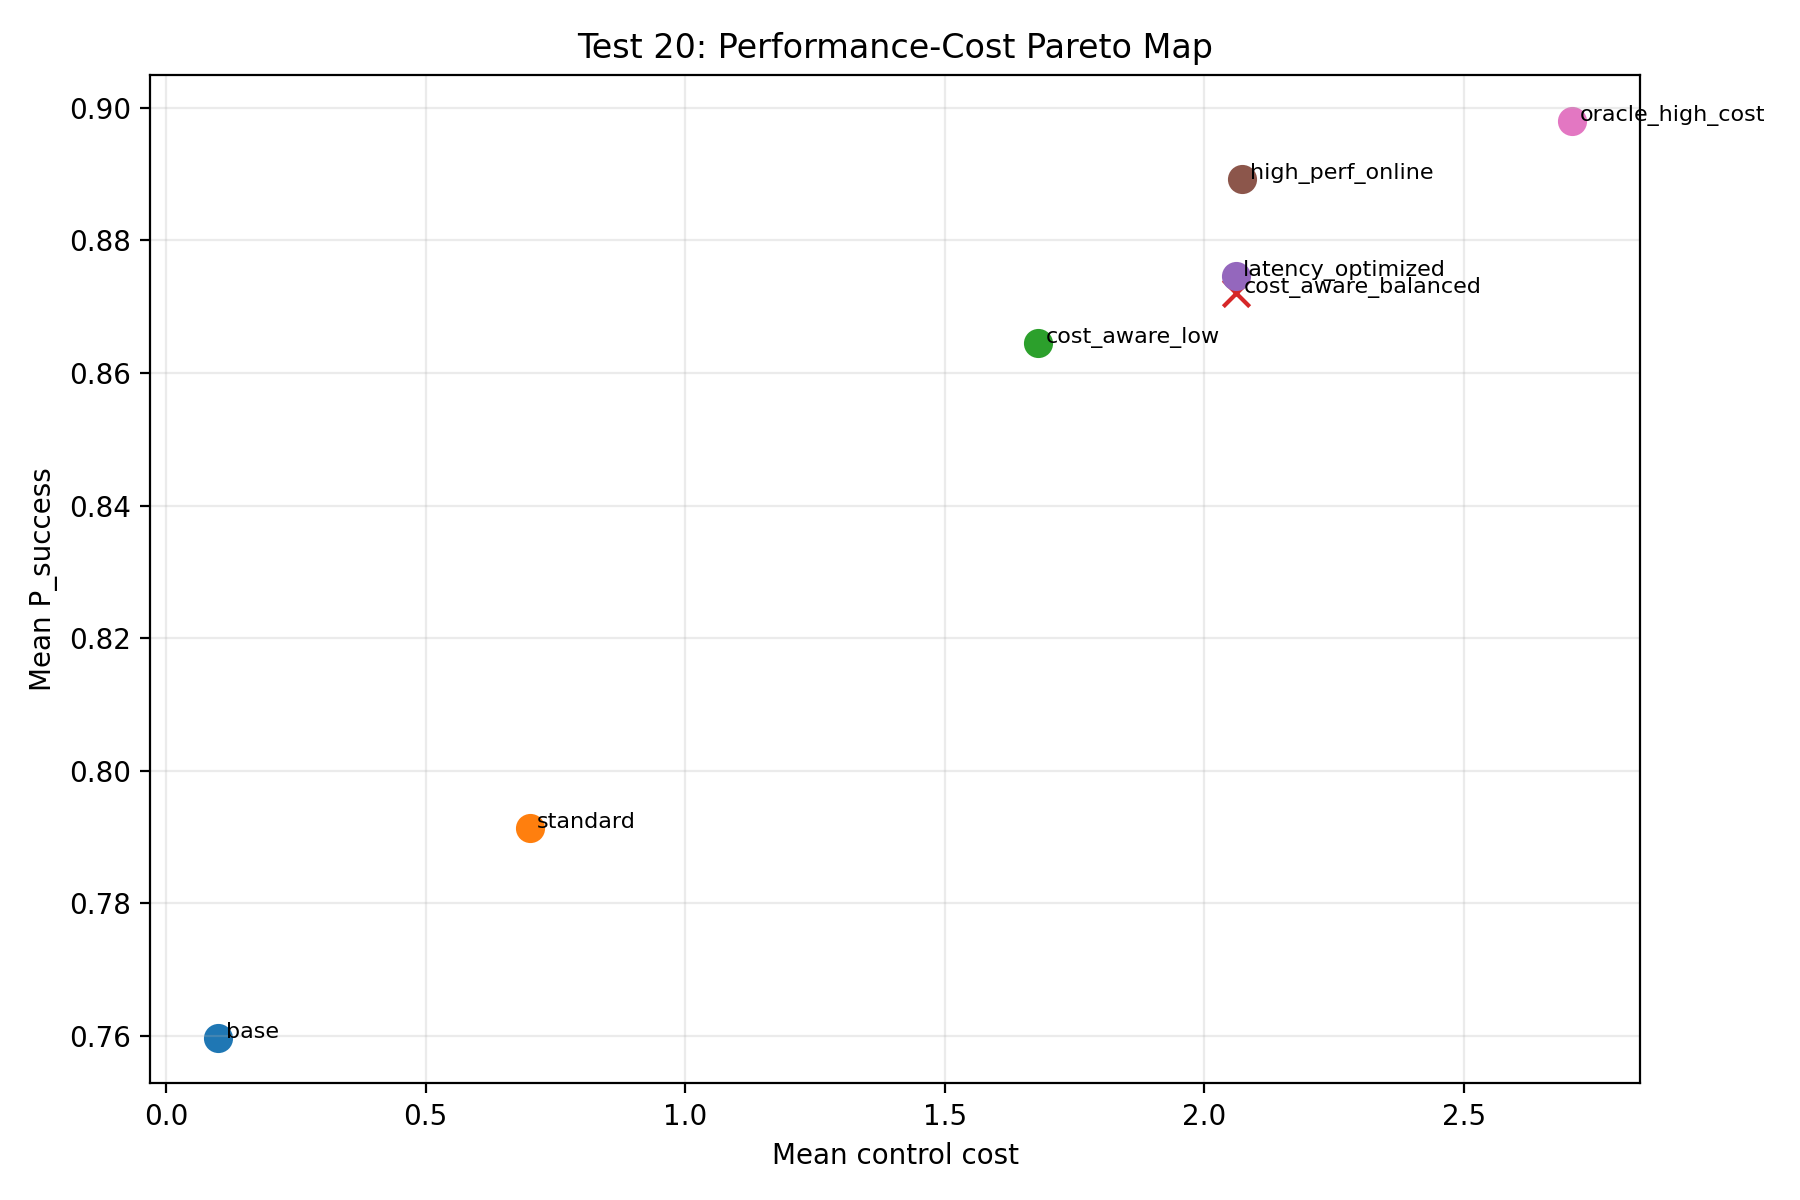
\includegraphics[width=0.75\linewidth]{figures/fig_test20_pareto.png}
\caption{Test 20: performance-cost Pareto map.}
\end{figure}

\subsection{Test 21: cost-interface boundary}

Test 21 находит критическую границу:
\[
U_{hp}=U_{ca},
\]
\[
\lambda^*=\frac{\Delta P_{hp}-\Delta P_{ca}}{ExtraCost_{hp}-ExtraCost_{ca}}.
\]
Главная boundary:
\[
\lambda^*\approx 0.0636.
\]
Если $\lambda<\lambda^*$, выгоднее high-performance. Если $\lambda>\lambda^*$, выгоднее cost-aware.

\begin{longtable}{p{6.6cm}rrp{3.3cm}}
\toprule
Boundary & Mean $\lambda^*$ & Median $\lambda^*$ & 95\% range \\
\midrule
\endfirsthead
\toprule
Boundary & Mean $\lambda^*$ & Median $\lambda^*$ & 95\% range \\
\midrule
\endhead
high\_perf\_online = cost\_aware\_balanced & 0.4652 & 0.3340 & [0.0668, 2.3900] \\
high\_perf\_online = cost\_aware\_low & 0.0636 & 0.0640 & [0.0240, 0.1121] \\
high\_perf\_online = latency\_optimized & 0.3720 & 0.2900 & [0.0306, 1.9437] \\
latency\_optimized = cost\_aware\_low & 0.0265 & 0.0267 & [0.0103, 0.0460] \\
oracle\_high\_cost = cost\_aware\_low & 0.0326 & 0.0328 & [0.0182, 0.0485] \\
oracle\_high\_cost = high\_perf\_online & 0.0153 & 0.0133 & [0.0011, 0.0384] \\
\bottomrule
\end{longtable}

Это можно записать как интерфейс переключения:
\[
B_{cost}:U_{hp}=U_{ca},
\]
\[
\boxed{I_{cost}:=B_{cost}\circ T(Control_{hp}\leftrightarrow Control_{ca})}.
\]

\begin{figure}[H]
\centering
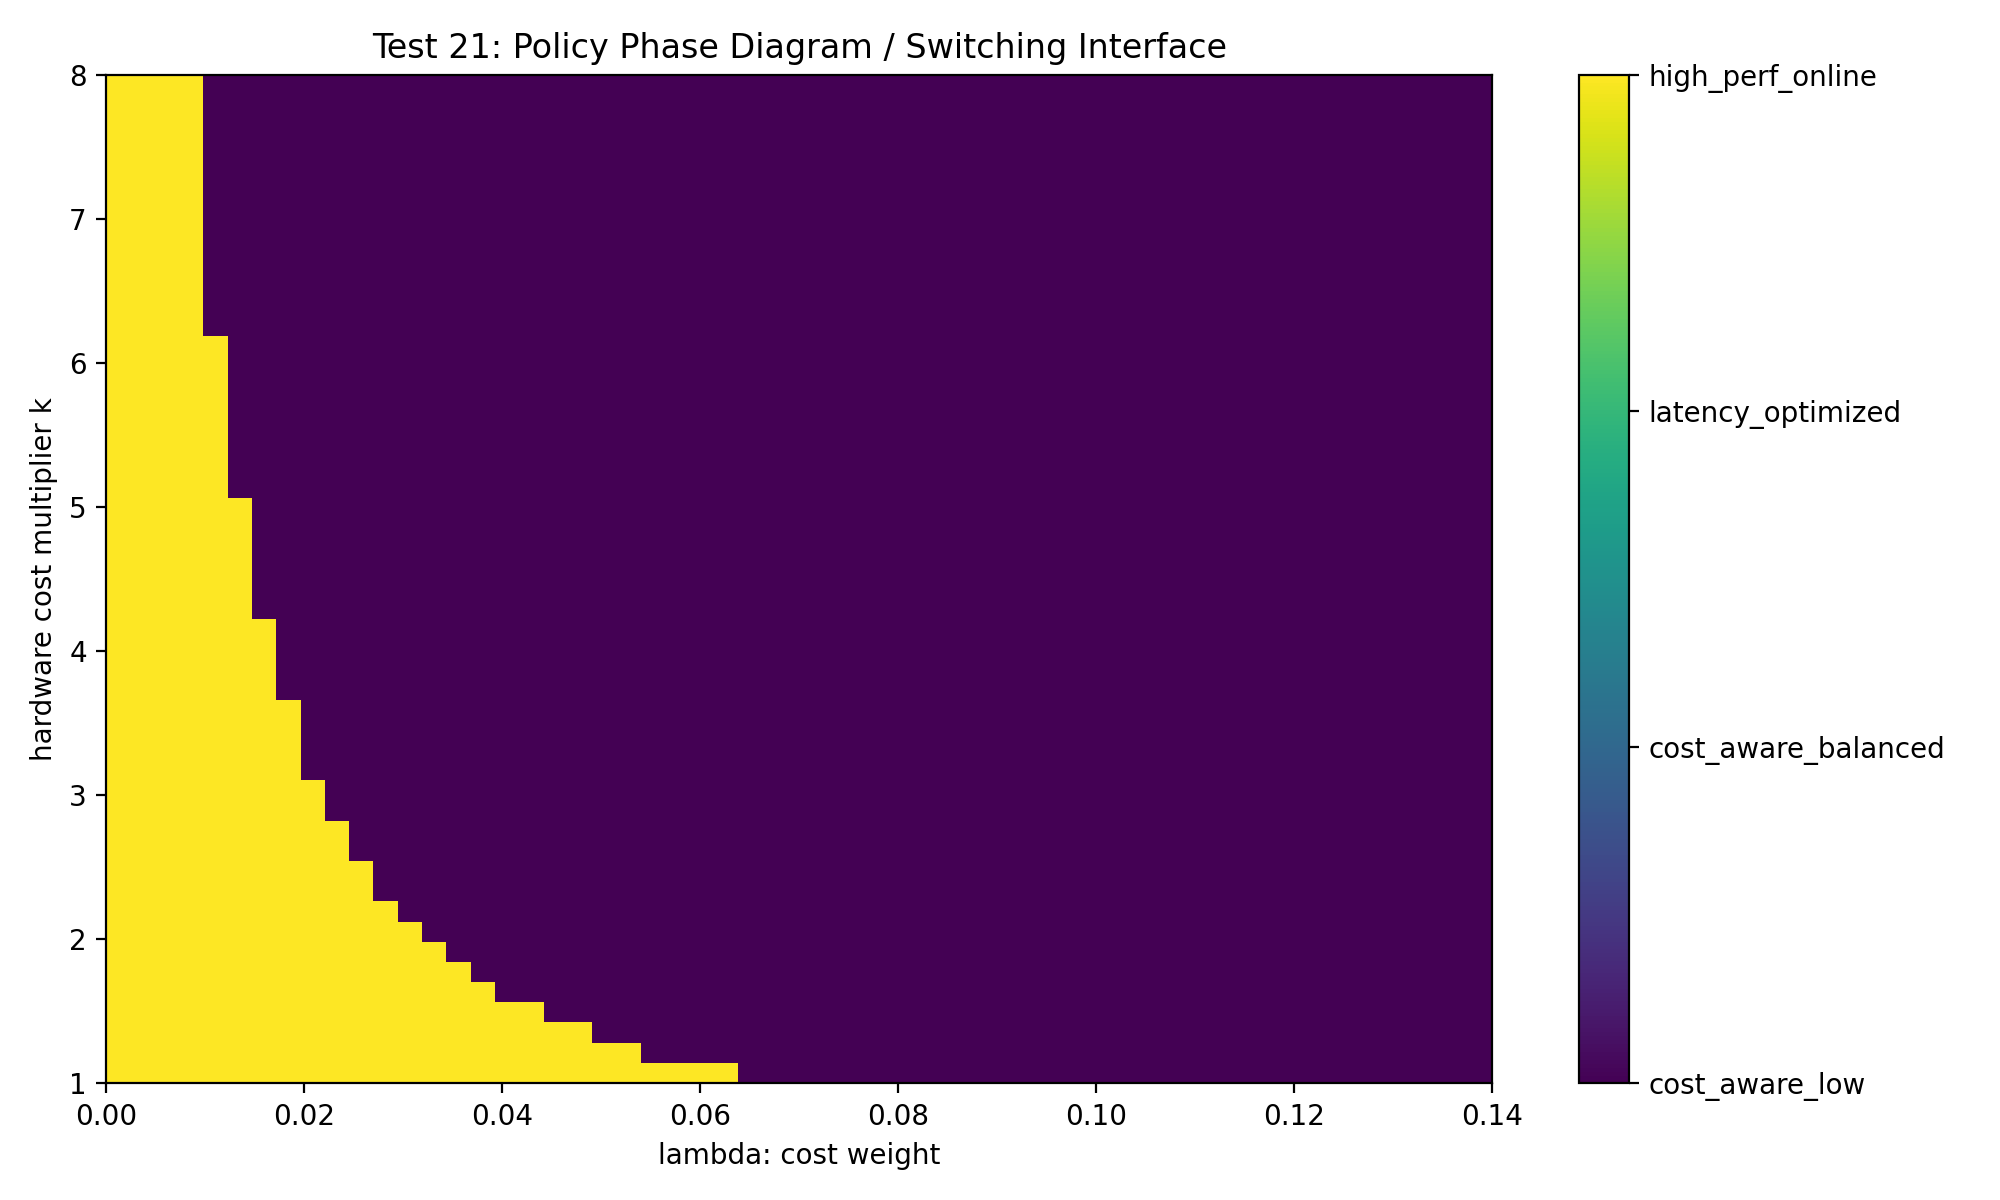
\includegraphics[width=0.82\linewidth]{figures/fig_test21_phase.png}
\caption{Test 21: policy phase diagram; boundary становится интерфейсом переключения режимов.}
\end{figure}

\subsection{Test 22: multi-objective boundary manifold}

Test 22 обобщает одну границу на многообразие границ. Для политики:
\[
O(policy)=(P,Cost,Safety,Latency,Robustness).
\]
Для вектора предпочтений:
\[
w=(w_P,w_C,w_S,w_L,w_R),
\]
\[
Score(policy;w)=w\cdot O(policy).
\]
Граница между двумя режимами:
\[
Score_i(w)=Score_j(w).
\]
Совокупность границ:
\[
\boxed{\mathcal M_{boundary}=\{{w:\arg\max_{policy}Score(policy;w)\ \text{изменяется}\}}}.
\]
Когда система использует это многообразие для переключения режимов, получаем:
\[
\boxed{I_{multi}:=\mathcal M_{boundary}\circ T(Control_i\leftrightarrow Control_j)}.
\]

\begin{longtable}{p{4.0cm}rrrrr}
\toprule
Policy & $P$ & Cost & Safety & Latency & Robustness \\
\midrule
\endfirsthead
\toprule
Policy & $P$ & Cost & Safety & Latency & Robustness \\
\midrule
\endhead
cost\_aware\_balanced & 0.677 & 0.352 & 0.830 & 0.353 & 0.811 \\
cost\_aware\_low & 0.646 & 0.533 & 0.887 & 0.589 & 0.841 \\
high\_perf\_online & 0.749 & 0.346 & 0.632 & 0.255 & 0.692 \\
latency\_optimized & 0.688 & 0.352 & 0.764 & 0.464 & 0.845 \\
oracle\_high\_cost & 0.786 & 0.044 & 0.593 & 0.031 & 0.836 \\
standard & 0.339 & 1.000 & 0.774 & 0.876 & 0.712 \\
\bottomrule
\end{longtable}

Winner share в sampled preference space:
\[
standard=0.608,\qquad cost\text{-}aware\ low=0.373.
\]

\begin{figure}[H]
\centering
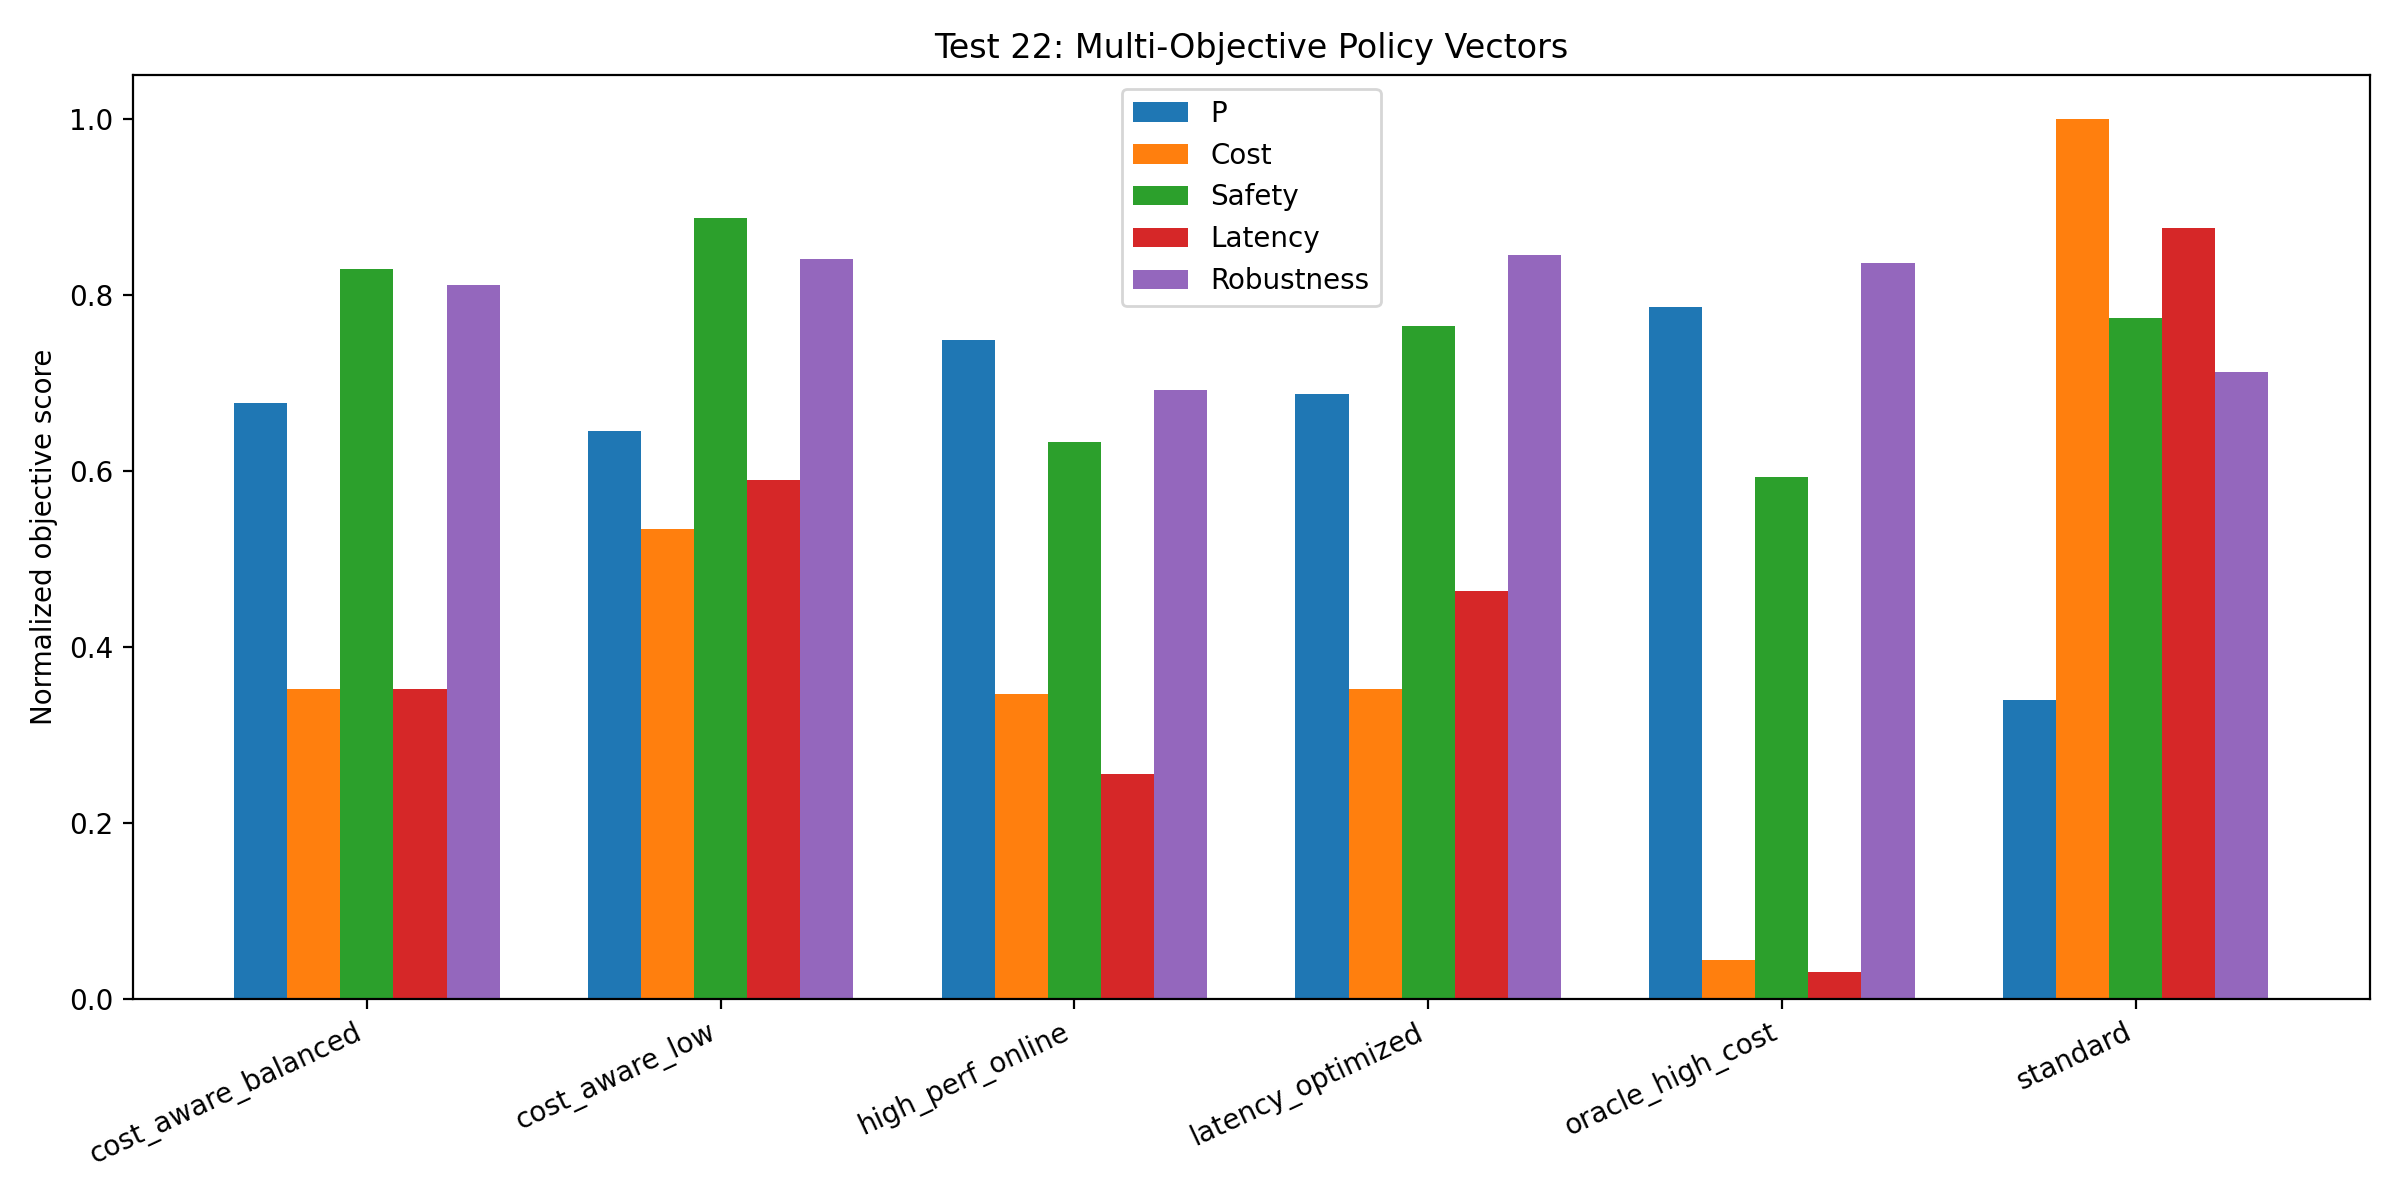
\includegraphics[width=0.82\linewidth]{figures/fig_test22_objectives.png}
\caption{Test 22: objective vectors по политикам управления.}
\end{figure}

\begin{figure}[H]
\centering
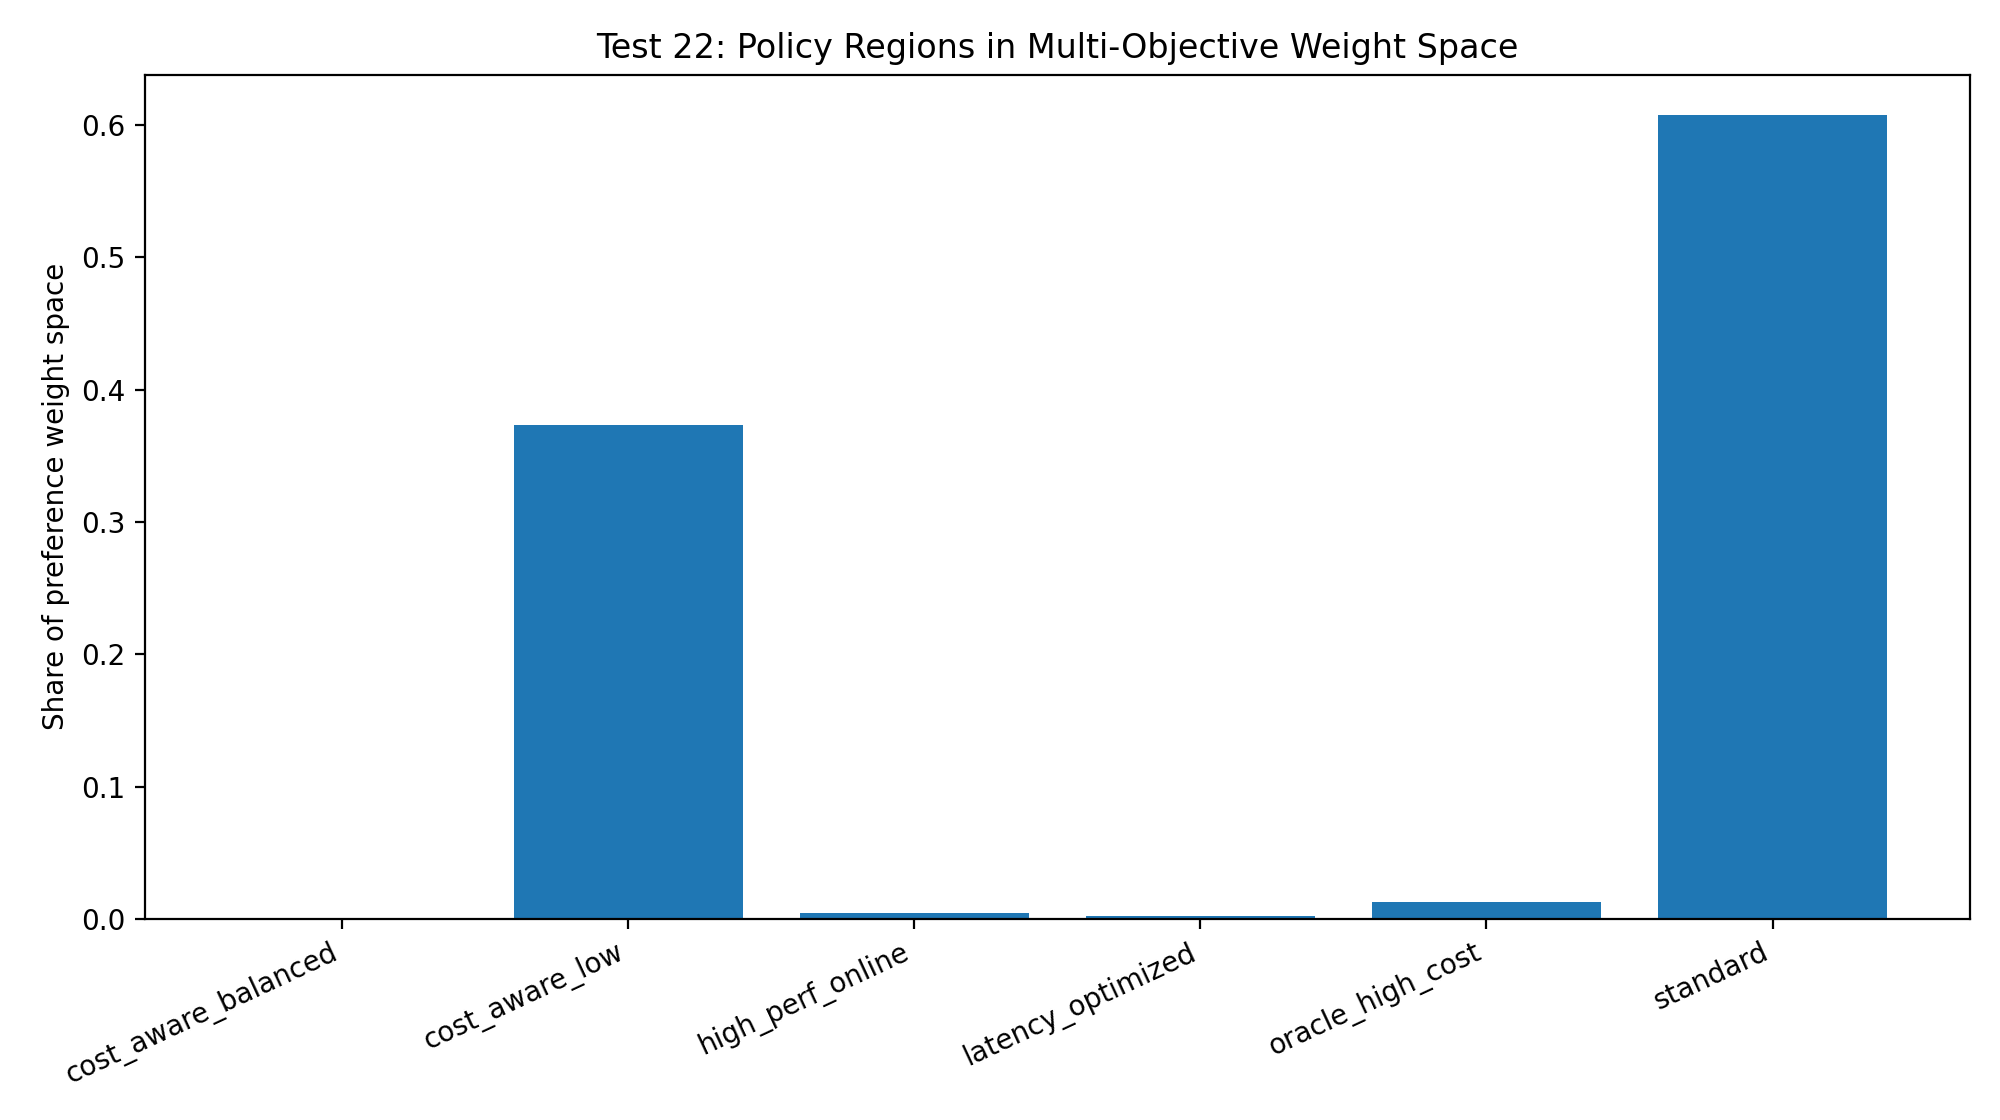
\includegraphics[width=0.78\linewidth]{figures/fig_test22_weights.png}
\caption{Test 22: доля пространства предпочтений, где политика является лучшей.}
\end{figure}

\begin{figure}[H]
\centering
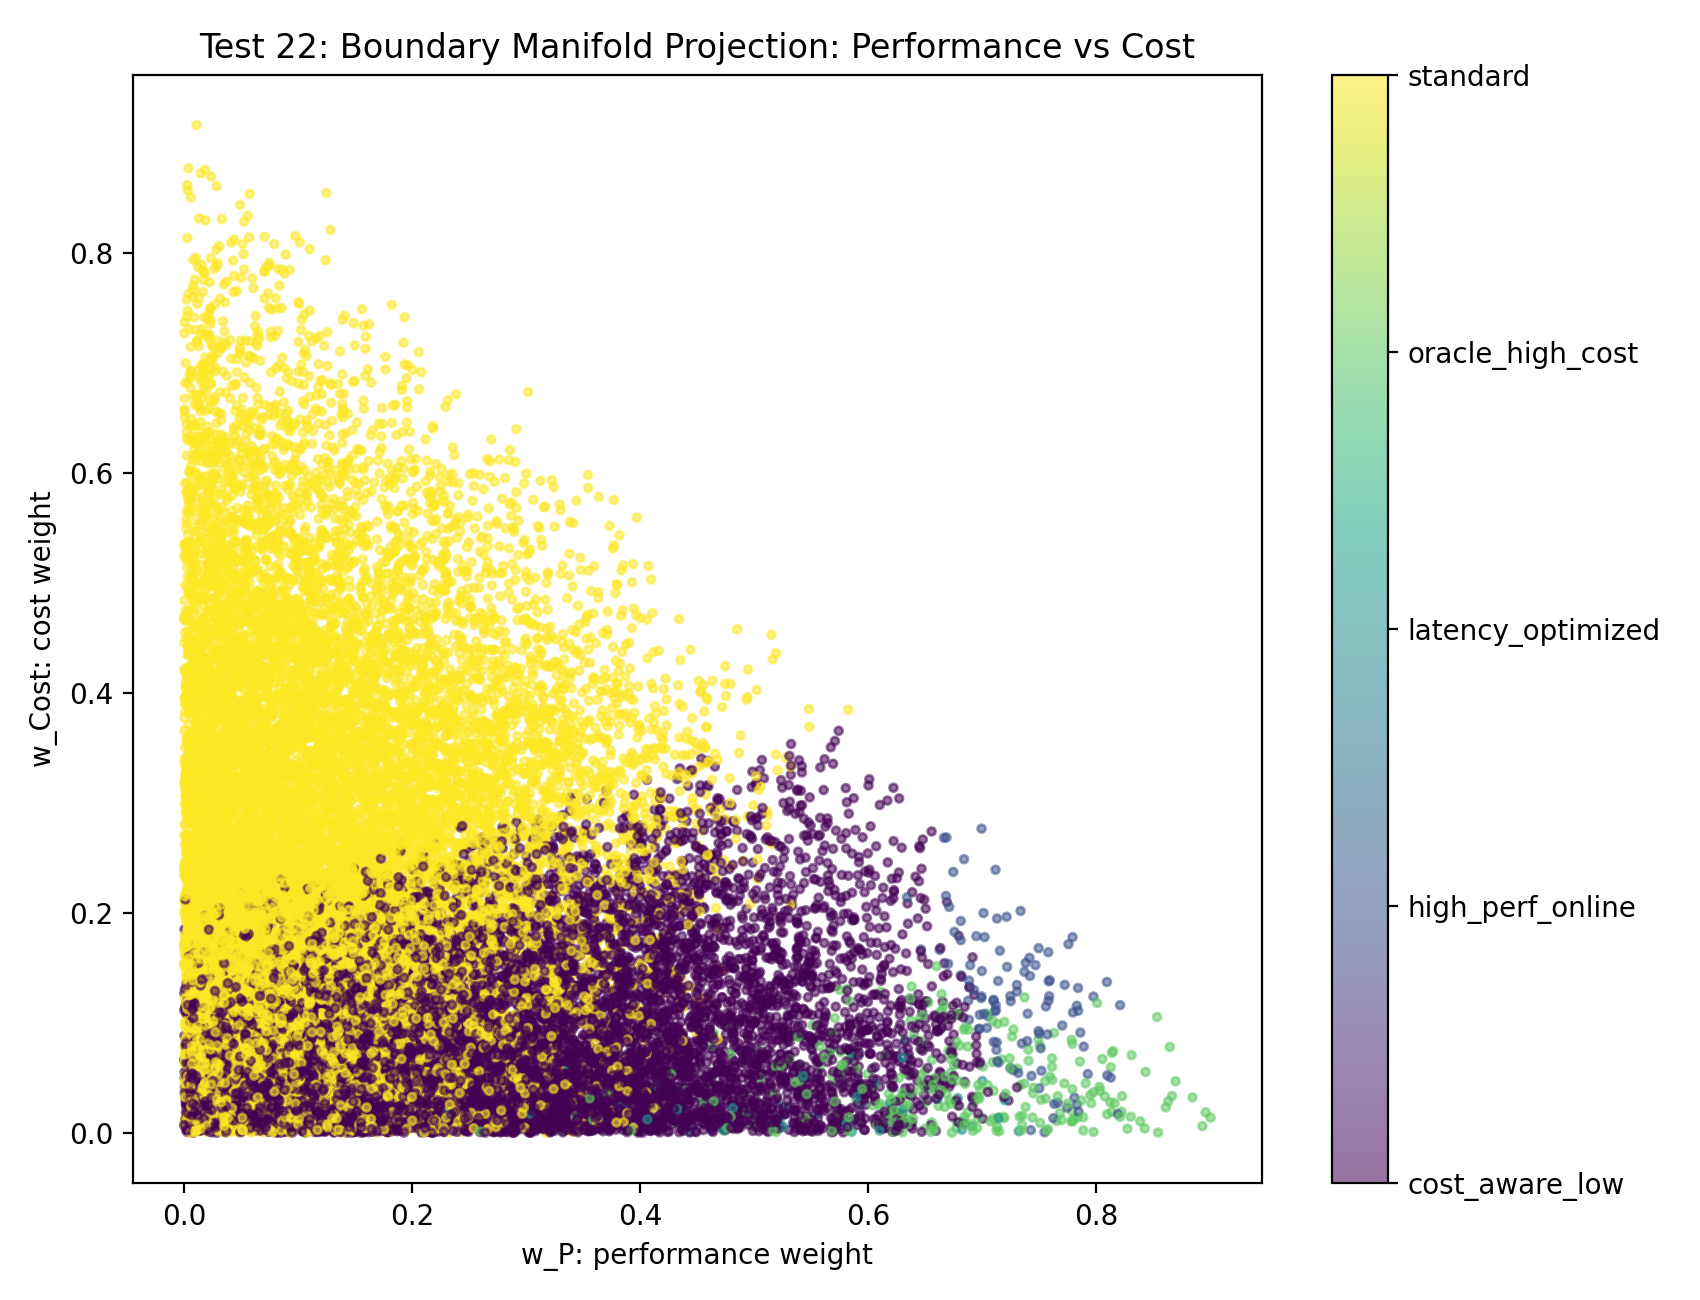
\includegraphics[width=0.74\linewidth]{figures/fig_test22_boundary_pc.png}
\caption{Test 22: проекция $\mathcal M_{boundary}$ на веса performance/cost.}
\end{figure}

\section{Интерпретация для Теории многообразных интерфейсов}

Tests 1--19 строят интерфейс как адаптивную систему управления состоянием:
\[
Input\Rightarrow Interpretation\Rightarrow ControlLayer\Rightarrow Output.
\]
Tests 20--22 добавляют пространство целей и границ. Теперь интерфейс не просто выбирает параметр, а выбирает режим из множества допустимых режимов:
\[
\{Control_i\}_{i\in\Lambda}.
\]
Смена режима происходит на границах:
\[
B_{ij}:Score_i(w)=Score_j(w).
\]
Их совокупность образует многообразие границ:
\[
\mathcal M_{boundary}=\bigcup_{i,j}B_{ij}.
\]
Полная формула:
\[
\boxed{\mathcal M_{boundary}\circ T(Control_i\leftrightarrow Control_j)\Rightarrow I_{multi}}
\]

\section{Главный вывод}

Вычислительная линия теперь имеет три уровня:
\[
\text{Level 1: adaptive control}\quad Tests\ 1--13,
\]
\[
\text{Level 2: noise-specific and drift-adaptive control}\quad Tests\ 14--19,
\]
\[
\text{Level 3: boundary-manifold control}\quad Tests\ 20--22.
\]

Сжатая итоговая формула:
\[
\boxed{
AutoInterface+NoiseInterpretation+CostBoundary+MultiObjectiveBoundaryManifold
\Rightarrow
ManifoldAdaptiveControl
}
\]

\section{Ограничения}

\begin{enumerate}[label=\arabic*.]
\item Это вычислительная валидация, а не лабораторное подтверждение.
\item Tests 20--22 используют синтетическую модель cost/safety/latency/robustness.
\item Нужна независимая реализация полной линии на Qiskit/Cirq/QuTiP или аналогичном backend.
\item Нужна hardware-specific калибровка стоимости управления.
\item Multi-objective boundary manifold пока является вычислительной моделью, а не измеренным физическим объектом.
\end{enumerate}

\section{Следующие шаги}

\begin{enumerate}[label=\arabic*.]
\item Зафиксировать Tests 1--22 как \textbf{Computational Validation Module 0.2}.
\item Подготовить английскую публикационную версию этого отчёта.
\item Сделать репозиторий с единым \texttt{run\_all\_tests.py} для расширенной линии 1--22.
\item Заменить synthetic cost/safety/latency на hardware-specific estimates.
\item После этого проектировать cloud-QPU protocol.
\end{enumerate}

\appendix
\section{Состав архива}

В архив входят:
\begin{itemize}
\item PDF и LaTeX исходник отчёта;
\item figures/ -- ключевые графики Tests 1--22;
\item data/ -- CSV/JSON/README summary-файлы;
\item test\_archives/ -- доступные архивы отдельных тестов в текущем рабочем наборе; ранняя линия Tests 1--11 отражена в сводной таблице и предыдущем отчёте v2.
\end{itemize}

\end{document}
